    \documentclass[11pt,
        usenames, % allows access to some tikz colors
        dvipsnames % more colors: https://en.wikibooks.org/wiki/LaTeX/Colors
    ]{report}
    \usepackage{
        amsmath,
        amssymb,
        fouriernc, % fourier font w/ new century book
        fancyhdr, % page styling
        lastpage, % footer fanciness
        hyperref, % various links
        setspace, % line spacing
        amsthm, % newtheorem and proof environment
        mathtools, % \Aboxed for boxing inside aligns, among others
        float, % Allow [H] figure env alignment
        enumerate, % Allow custom enumerate numbering
        graphicx, % allow includegraphics with more filetypes
        wasysym, % \smiley!
        upgreek, % \upmu for \mum macro
        listings, % writing TrueType fonts and including code prettily
        tikz, % drawing things
        booktabs, % \bottomrule instead of hline apparently
        cancel % can cancel things out!
    }
    \usepackage[margin=1in]{geometry} % page geometry
    \usepackage[
        labelfont=bf, % caption names are labeled in bold
        font=scriptsize % smaller font for captions
    ]{caption}
    \usepackage[font=scriptsize]{subcaption} % subfigures

    \newcommand*{\scinot}[2]{#1\times10^{#2}}
    \newcommand*{\bra}[1]{\left<#1\right|}
    \newcommand*{\ket}[1]{\left|#1\right>}
    \newcommand*{\dotp}[2]{\left<#1\,\middle|\,#2\right>}
    \newcommand*{\rd}[2]{\frac{\mathrm{d}#1}{\mathrm{d}#2}}
    \newcommand*{\pd}[2]{\frac{\partial#1}{\partial#2}}
    \newcommand*{\rtd}[2]{\frac{\mathrm{d}^2#1}{\mathrm{d}#2^2}}
    \newcommand*{\ptd}[2]{\frac{\partial^2 #1}{\partial#2^2}}
    \newcommand*{\md}[2]{\frac{\mathrm{D}#1}{\mathrm{D}#2}}
    \newcommand*{\norm}[1]{\left|\left|#1\right|\right|}
    \newcommand*{\abs}[1]{\left|#1\right|}
    \newcommand*{\pvec}[1]{\vec{#1}^{\,\prime}}
    \newcommand*{\svec}[1]{\vec{#1}\;\!}
    \newcommand*{\bm}[1]{\boldsymbol{\mathbf{#1}}}
    \newcommand*{\expvalue}[1]{\left<#1\right>}
    \newcommand*{\ang}[0]{\text{\AA}}
    \newcommand*{\mum}[0]{\upmu \mathrm{m}}
    \newcommand*{\at}[1]{\left.#1\right|}

    \newtheorem{theorem}{Theorem}[section]

    \let\Re\undefined
    \let\Im\undefined
    \DeclareMathOperator{\Res}{Res}
    \DeclareMathOperator{\Re}{Re}
    \DeclareMathOperator{\Im}{Im}
    \DeclareMathOperator{\Log}{Log}
    \DeclareMathOperator{\Arg}{Arg}
    \DeclareMathOperator{\Tr}{Tr}
    \DeclareMathOperator{\E}{E}
    \DeclareMathOperator{\Var}{Var}
    \DeclareMathOperator*{\argmin}{argmin}
    \DeclareMathOperator*{\argmax}{argmax}
    \DeclareMathOperator{\sgn}{sgn}
    \DeclareMathOperator{\diag}{diag\;}

    \DeclarePairedDelimiter\p{\lparen}{\rparen}
    \DeclarePairedDelimiter\s{\lbrack}{\rbrack}
    \DeclarePairedDelimiter\z{\lbrace}{\rbrace}

    % \everymath{\displaystyle} % biggify limits of inline sums and integrals
    \tikzstyle{circ} % usage: \node[circ, placement] (label) {text};
        = [draw, circle, fill=white, node distance=3cm, minimum height=2em]
    \definecolor{commentgreen}{rgb}{0,0.6,0}
    \lstset{
        basicstyle=\ttfamily\footnotesize,
        frame=single,
        numbers=left,
        showstringspaces=false,
        keywordstyle=\color{blue},
        stringstyle=\color{purple},
        commentstyle=\color{commentgreen},
        morecomment=[l][\color{magenta}]{\#}
    }

\begin{document}

\def\Snospace~{\S{}} % hack to remove the space left after autorefs
\renewcommand*{\sectionautorefname}{\Snospace}
\renewcommand*{\appendixautorefname}{\Snospace}
\renewcommand*{\figureautorefname}{Fig.}
\renewcommand*{\equationautorefname}{Eq.}
\renewcommand*{\tableautorefname}{Tab.}

\onehalfspacing

\pagestyle{fancy}
\rfoot{Yubo Su}
\cfoot{\thepage/\pageref{LastPage}}

\title{Research Notes}
\author{Yubo Su}

\maketitle

\tableofcontents

\newpage

\chapter{Preliminary Problems}

To get an intuition for how Dedalus and fluid mechanics works, we will solve
some toy problems. Recall fluid equations in the presence of a uniform
gravitational field $\vec{g} = -g\hat{z}$:
\begin{equation}
    \begin{split}
        \rd{\rho}{t} + \vec{\nabla} \cdot \vec{u} &= 0,\\
        \rd{\vec{u}}{t} + \frac{\vec{\nabla}P}{\rho} - \vec{g} &= 0.
    \end{split}\label{eq:fluid_eq}
\end{equation}

In the incompressible limit, $\rd{\rho}{t} = 0$, which implies $\vec{\nabla}
\cdot \vec{u} = 0$. We use subscripts to indicate perturbed quantities, $Q_0$ is
background and $Q_1$ is perturbed. We will generally use $\vec{u}_0 = 0$ unless
otherwise noted. We will also generally assume symmetry along all axes except
$z$ the vertical axis.

In the incompressible limit, the fluid equations become
\begin{equation}
    \begin{split}
        \vec{\nabla} \cdot \vec{u}_1 &= 0,\\
        \pd{\rho_1}{t} + u_{1z}\pd{\rho_0}{z} &= 0,\\
        \pd{\vec{u}_1}{t} + \frac{1}{\rho_0}\vec{\nabla}P_1
            + \frac{\rho_1 g \hat{z}}{\rho_0} &= 0.
    \end{split}\label{eq:lin.incomp}
\end{equation}
We have used $\vec{\nabla}P_0 = -\rho_0 g \hat{z}$ in the absence of
perturbations.

\section{Incompressible, No Gravity}

We note that in the no gravity limit that $\rho_1$ does not have an effect on
other dynamical variables, so the equations of motion we must solve are
\begin{equation}
    \begin{split}
        \vec{\nabla} \cdot \vec{u}_1 &= 0,\\
        \pd{\vec{u}_1}{t} + \frac{\vec{\nabla}P_1}{\rho_0} &= 0.
    \end{split}\label{eq:lin.no_g_eom}
\end{equation}
We can take the divergence of the momentum equation and substitute the
continuity equation to get $\nabla^2 P = 0$. This is a Laplace equation, which
we've solved countless times. Imposing periodic boundary conditions in the $x$
direction and $P_1(z = L) = 0, P_1(z = 0) = \mathcal{P}(x, t)$, we obtain
eigenfunctions
\begin{equation}
    \begin{split}
        P_{1, n}(x, z, t) &=
            \frac{\mathcal{P}_n(t)}{\sinh(k_nL)}e^{ik_nx}\sinh\p*{k_n(L - z)},\\
        u_{1x, n}(x, z, t) &=
            \int\limits^t -\frac{1}{\rho_0}\pd{P_{1, n}}{x}\;\mathrm{d}t,\\
        u_{1z, n}(x, z, t) &=
            \int\limits^t -\frac{1}{\rho_0}\pd{P_{1, n}}{z}\;\mathrm{d}t.
    \end{split}\label{eq:incomp_nog}
\end{equation}
We define $k_n = \frac{2\pi n}{L}, n \in [0, L - 1]$ and $\mathcal{P}(x, t) =
\sum\limits_n \mathcal{P}_n(t)e^{ik_nx}$.

Thus, if we impose BCs $\mathcal{P}(x, t) = \sin \frac{2\pi x}{L}$ and start
with initial conditions such that all quantities are zero, we would expect after
transients die out that
\begin{equation}
    \begin{split}
        P(x, z, t) &= \frac{\sin \frac{2\pi x}{L}}{\sinh 2\pi}
            \sinh \p*{2\pi \frac{L - z}{L}},\\
        u_{1x}(x, z, t) &= -\frac{2\pi t}{L\rho_0}
            \frac{\cos \frac{2\pi x}{L}}{\sinh 2\pi}\sinh \p*{2\pi \frac{L -
                z}{L}},\\
        u_{1z}(x, z, t) &= +\frac{2\pi t}{L\rho_0}
            \frac{\sin \frac{2\pi z}{L}}{\sinh 2\pi}\cosh \p*{2\pi \frac{L -
                z}{L}}.
    \end{split}\label{eq:incomp_nog_sol}
\end{equation}
This is in good agreement with the results, presented in \autoref{fig:no_g}.
Note that $P$ is constant while $\vec{u}$ increases linearly in time, and we
observe the expected $\sim \sin x \sinh \frac{L - z}{z}$ dependence.

\begin{figure}[!h]
    \centering
    \begin{subfigure}{0.3\textwidth}
        \centering
        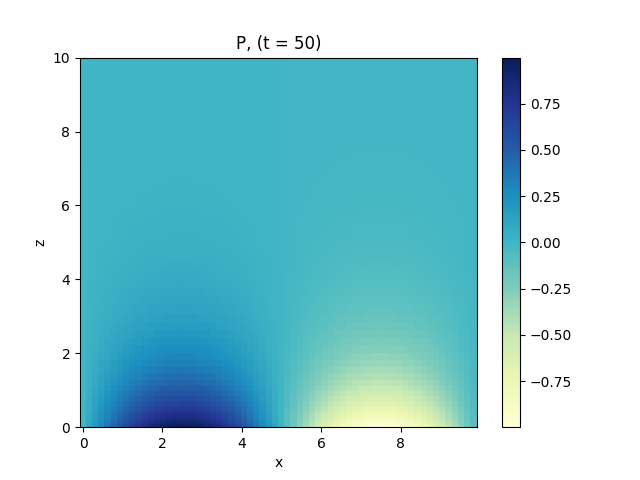
\includegraphics[width=\textwidth]{../sims/prelim/no_g/no_g_P_t50.png}
    \end{subfigure}
    \begin{subfigure}{0.3\textwidth}
        \centering
        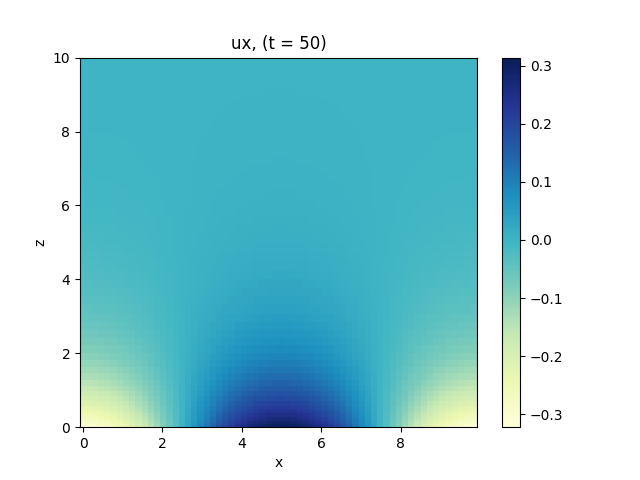
\includegraphics[width=\textwidth]{../sims/prelim/no_g/no_g_ux_t50.png}
    \end{subfigure}
    \begin{subfigure}{0.3\textwidth}
        \centering
        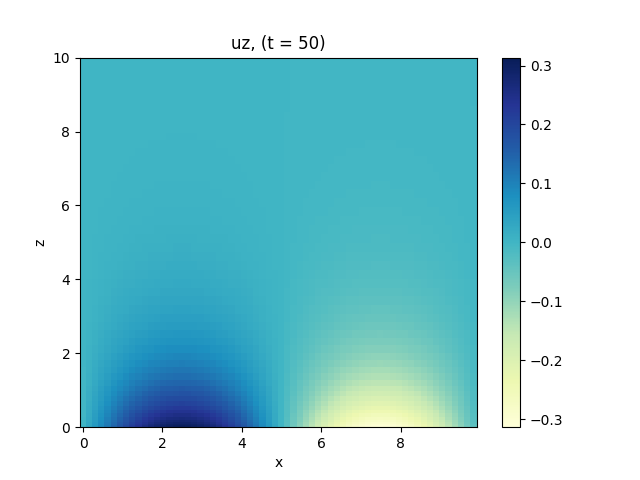
\includegraphics[width=\textwidth]{../sims/prelim/no_g/no_g_uz_t50.png}
    \end{subfigure}

    \begin{subfigure}{0.3\textwidth}
        \centering
        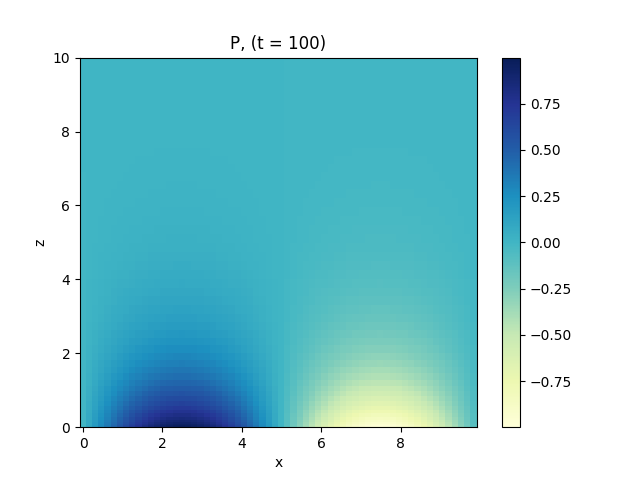
\includegraphics[width=\textwidth]{../sims/prelim/no_g/no_g_P_t100.png}
    \end{subfigure}
    \begin{subfigure}{0.3\textwidth}
        \centering
        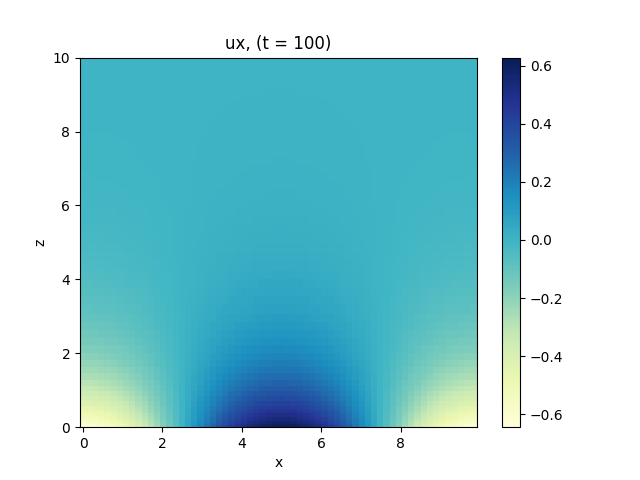
\includegraphics[width=\textwidth]{../sims/prelim/no_g/no_g_ux_t100.png}
    \end{subfigure}
    \begin{subfigure}{0.3\textwidth}
        \centering
        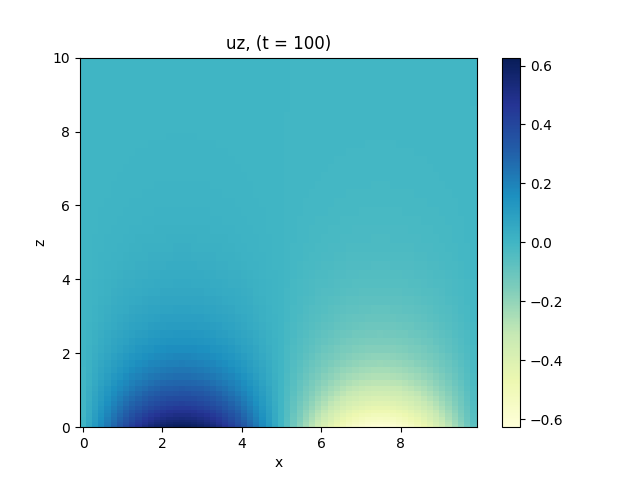
\includegraphics[width=\textwidth]{../sims/prelim/no_g/no_g_uz_t100.png}
    \end{subfigure}
    \caption{$P, u_x, u_z$ at $t = 0.5$ and $t = 1$ for $\rho_0 = 1$.
    }\label{fig:no_g}
\end{figure}

It is worth noting that, since our \autoref{eq:lin.no_g_eom} reduced to a Laplace
equation, we needed two $z$ BCs and two $x$ BCs (periodic BCs amount to equating
the value and derivative of the function). This is in agreement with the
observation that the original \autoref{eq:lin.no_g_eom} had two derivatives in
$x, z$ apiece, so we needed two BCs each.

\chapter{2D Wave Breaking in Atmospheres}

The goal of this will be to lay out a formalism that can reproduce Sutherland et
al.~2011\footnote{DOI:10.1175/JAS-D-11--097.1} and also investigate driven
oscillations versus the breaking of a single wave packet. This represents wave
breaking in the atmosphere.

\section{Dynamical Setup}

We adopt notation where $q_0$ is the background quantity and $q_1$ is the
perturbed quantity from the propagating wave.

The fluid equations are
\begin{subequations}\label{se:fl_eq}
    \begin{align}
        \pd{\rho}{t} + \vec{\nabla} \cdot \rho \vec{u} &= 0,
            \label{eq:fl_eq.cont}\\
        \rd{\vec{u}}{t} &= -\vec{\nabla}\frac{P}{\rho} - g\hat{z},
            \label{eq:fl_eq.mom}
    \end{align}
\end{subequations}
where we will take gravity to be uniform throughout the domain of interest. We
will study for no background flow $\vec{u}_0 = 0$ and in the presence of
stratification $\rho_0 \propto e^{-z/H}$. In the absence of any perturbations it
is then easy to show that $\rd{P_0}{z} = -\rho_0 g$.

\subsection{Linear, Incompressible}

\subsubsection{Solution for Arbitrary Stratification}

First, we solve the incompressible case $c_s^2 \to \infty, \vec{\nabla} \cdot
\vec{u} = 0$ in the linear regime. For funsies, we solve for arbitrary
stratification first. The fluid equations to first order reduce to
\begin{equation}
    \begin{split}
        \pd{\rho_1}{t} + \p*{\vec{u}_1 \cdot \vec{\nabla}}\rho_0 &= 0,\\
        \vec{\nabla} \cdot \vec{u}_1 &= 0,\\
        \pd{\vec{u}_1}{t} &= -\frac{\vec{\nabla}P_1}{\rho_0}
            - P_1 \vec{\nabla}\frac{1}{\rho_0}
    \end{split}\label{eq:lin_incomp}
\end{equation}
We expect there to be some $z$ dependence in the amplitude, so we substitute
variables of form $e^{i(kx - \omega t)}$ and do not specify the $z$ dependence.
This gives us
\begin{equation}
    \begin{split}
        -i\omega \rho_1 - u_{1z}\pd{\rho_0}{z} &= 0,\\
        iku_{1x} + \pd{u_{1z}}{z} &= 0,\\
        -iw u_{1x} + \frac{ik_x P_1}{\rho_0} &= 0,\\
        -iw u_{1z} + \frac{1}{\rho_0}\pd{P_1}{z} +
            \frac{\rho_1}{\rho_0^2}\pd{P_0}{z} &= 0.
    \end{split}
\end{equation}
We substitute $N^2 = -\frac{g}{\rho_0}\pd{\rho_0}{z}$ and $\pd{P_0}{z} = -\rho
g$ to obtain
\begin{subequations}
    \begin{align}
        -i\omega \rho_1 - u_{1z}\frac{\rho_0N^2}{g} &= 0,\label{eq:lin.cont}\\
        iku_{1x} + \pd{u_{1z}}{z} &= 0,\label{eq:lin.div}\\
        -iw u_{1x} + \frac{ik_x P_1}{\rho_0} &= 0,\label{eq:lin.mom_x}\\
        -iw u_{1z} + \frac{1}{\rho_0}\pd{P_1}{z} +
            \frac{\rho_1g}{\rho_0} &= 0.\label{eq:lin.mom_z}
    \end{align}
\end{subequations}
Eliminating $u_{1x}$ by substituting~\eqref{eq:lin.div}
into~\eqref{eq:lin.mom_x} and $\rho_1$ by substituting~\eqref{eq:lin.cont}
into~\eqref{eq:lin.mom_z} give
\begin{subequations}
    \begin{align}
        i\omega \pd{u_{1z}}{z} + \frac{k_x^2 P_1}{\rho_0} &= 0,
            \label{eq:lin.eq1}\\
        \p*{\omega^2 - N^2 }u_{1z} + \frac{i\omega}{\rho_0}\pd{P_1}{z} &= 0.
            \label{eq:lin.eq2}
    \end{align}
\end{subequations}
Finally, we multiply~\eqref{eq:lin.eq1} with $\rho_0$ and differentiate
$\mathrm{d}z$ and combine with~\eqref{eq:lin.eq2} to give
\begin{equation}
    \rtd{u_{1z}}{z} + \frac{1}{\rho_0}\pd{\rho_0}{z}\pd{u_{1z}}{z}
        + k_x^2\p*{\frac{N^2}{\omega^2} - 1}u_{1z} = 0.\label{eq:lin.incomp.gen}
\end{equation}

\subsubsection{Introduce Stratification}

With stratification $\rho \propto e^{-z/H}$ \autoref{eq:lin.incomp.gen} clearly
has exponential solutions $e^{\kappa z}$ for
\begin{equation}
    \kappa^2 - \frac{\kappa}{H} + k_x^2\p*{\frac{N^2}{\omega^2} - 1} = 0.
\end{equation}

We permit complex $\kappa = -\frac{1}{2H} + ik_z$, and from the above clearly
\begin{align}
    k_z^2 &= -\frac{1}{4H^2} + k_x^2\p*{\frac{N^2}{\omega^2} - 1},\nonumber\\
    \omega^2 &= \frac{N^2k_x^2}{k_x^2 + k_z^2 + \frac{1}{4H^2}}.
\end{align}

\subsection{Developing the Anelastic/Boussinesq Approximations}

Let's relax the incompressibility constraint (we will expand the continuity
equation to first order, but the momentum equation will merit a separate
treatment):
\begin{equation}
    \begin{split}
        \pd{\rho_1}{t} + \vec{\nabla} \cdot \p*{\rho_0 \vec{u}_1} &= 0,\\
        \pd{\vec{u}_1}{t} &= -\frac{\vec{\nabla}P}{\rho} - \vec{g}.
    \end{split}
\end{equation}
Suppose we are interested in phenomena with characteristic length scale $L$ and
time scale $\tau$. Let's first examine the relative magnitudes of the terms in
the continuity equation
\begin{equation*}
    \frac{\rho_1}{\tau} + \frac{\rho_0 \abs{u_1}}{L} = 0.
\end{equation*}
Thus, if we are interested in time scales $\tau \gg
\frac{\rho_1}{\rho_0}\frac{L}{\abs{u_1}}$ then we neglect the first term, the
time derivative. This corresponds to making the perturbation incompressible;
note that $\pd{\rho_1}{t} \approx \rd{\rho_1}{t}$ to first order, so we drop the
high frequency restoring forces in the perturbation.

For the momentum equation, we instead first manipulate to first order
\begin{align}
    -\frac{\vec{\nabla}P}{\rho} - \vec{g}
        &= -\frac{\vec{\nabla}P_0}{\rho} - \frac{\vec{\nabla}P_1}{\rho_0}
            - \vec{g},\nonumber\\
        &= - \frac{\vec{\nabla}P_1}{\rho_0} +
            \p*{\frac{\rho_0}{\rho} - 1}\vec{g},\nonumber\\
        &= -\vec{\nabla}\p*{\frac{P_1}{\rho_0}}
            - \frac{P_1}{\rho_0^2}\vec{\nabla}\rho_0
            - \frac{\rho_1}{\rho_0}\vec{g}.
\end{align}

We now have three equations for four variables, $\vec{u}_1, \rho_1, P_1$. We
must introduce a fourth equation, a thermodynamic equation. For an adiabatic
process $P\rho^{-\gamma} \propto P^{1-\gamma}T^\gamma$ is constant. We thus
introduce the concept of the \emph{potential temperature}
\begin{equation}
    \theta = T\p*{\frac{P_0}{P}}^\kappa.
        \label{eq:pot_temp}
\end{equation}
For an adiabatic process, $\rd{\theta}{t} = 0$. Motivated by this, we use
\begin{equation}
    \begin{split}
        \pd{1}{\rho_0}\pd{\rho_0}{z} &= \frac{1}{\gamma P_0}\pd{P_0}{z}
            - \frac{1}{\theta_0}\pd{\theta_0}{z},\\
        \frac{\rho_1}{\rho_0} &= \frac{1}{\gamma} \frac{P_1}{P_0}
            - \frac{\theta_1}{\theta_0},
    \end{split}
\end{equation}
to give the momentum equation form
\begin{equation}
    \rd{\vec{u}_1}{t} = -\vec{\nabla}\p*{\frac{P_1}{\rho_0}}
        + \frac{P_1}{\rho_0}\p*{\frac{1}{\theta_0}\vec{\nabla}\theta_0}
        + \vec{g} \frac{\theta_1}{\theta_0}.\label{eq:mom_unsimp}
\end{equation}

We also recognize $N^2 = \frac{g}{\theta_0}\pd{\theta_0}{z}$. We now do the same
trick where we consider dynamics on length scale $D$ and compare the first and
second terms in \autoref{eq:mom_unsimp}. Their ratio is $\frac{N^2 D}{g}$, and
so as $N^2 \ll \frac{g}{D}$ the freefall time we neglect the second term.

The anelastic fluid equations thus read
\begin{equation}
    \begin{split}
        \vec{\nabla} \cdot \p*{\rho_0\vec{u}} &= 0,\\
        \pd{\vec{u}_1}{t} + \vec{\nabla}\p*{\frac{P_1}{\rho_0}}
            - \vec{g}\frac{\theta_1}{\theta_0} &= 0,\\
        \pd{\theta_1}{t} + \p*{\vec{u} \cdot \vec{\nabla}}\theta_0 &= 0.
    \end{split}\label{eq:lin_anelastic}
\end{equation}

The Boussinesq equations are obtained from these in the limit where $H \gg D$
the relevant length scale, thus we allow $\rho_0$ to be approximately constant.

\subsection{Anelastic Solution}

We simply substitute $e^{i(\vec{k} \cdot \vec{r} - \omega t)}$ into
\autoref{eq:lin_anelastic} with $\rho_0 \propto e^{-z/H}$ and obtain
\begin{equation}
    \begin{bmatrix}
        0 & 0 & ik_x\rho_0 & ik_z \rho_0 - \frac{\rho_0}{H}\\
        0 & -i\omega & 0 & \frac{N^2\theta_0}{g}\\
        \frac{ik_x}{\rho_0} & 0 & -i\omega & 0\\
        \frac{ik_z}{\rho_0} + \frac{1}{\rho_0 H} & -\frac{g}{\theta_0}
            & 0 & -i\omega
    \end{bmatrix} \begin{bmatrix}
        P_1 \\ \theta_1 \\ u_{1x} \\ u_{1z}
    \end{bmatrix} = 0.
\end{equation}
Taking the determinant of this matrix produces
\begin{align}
    -k_x^2\p*{-N^2 + \omega^2} + \p*{ik_z - \frac{1}{H}}
        \p*{ik_z + \frac{1}{H}}\omega^2 &= 0,\nonumber\\
    \frac{N^2k_x^2}{k_x^2 + k_z^2 + \frac{1}{4H^2}} &= \omega^2.
\end{align}

\section{Boundary Conditions}

\subsection{Incompressible}

We must bound this to a finite domain. We choose periodic boundary conditions in
$x$ with total length $L_x$, $x \in \s*{-\frac{L}{2}, \frac{L}{2}}$. We choose
$z$ dimension to have total length $L_z$, $z \in [0, L_z]$.

To set up the boundary condition at $z = 0$, we recall that gravity waves in an
atmosphere with $e^{-z/H}$ profile have form
\begin{equation}
    u_{1z} \propto e^{\frac{z}{2H}}e^{i\p*{k_xx + k_zz - \omega t}}.
        \label{eq:bc_below}
\end{equation}
We will take Boussinesq/WKB approximation $H \to 0$, reasonable in the linear
regime, to simplify the BCs. Then $\rho_1 = 0$ (reasonable in the incompressible
limit), $u_{1x} = -\frac{k_z}{k_x}u_{1z}$ and $P_1 = -\frac{\omega
\rho_0}{k_z}u_{1z}$, from the linearized incompressible equations.

The boundary condition at $z = L_z$ is much harder to determine. It is clear
that $\vec{u}_1(z = \infty) = \rho_1(z = \infty) = 0$, and for $L_z \gg H$ this
would be a reasonable approximation, if simply because we expect the majority of
the wave to dissipate via turbulent dissipation as $z$ reaches many $H$. We will
simply choose the BC to be many multiples of $H$. We can solve with both a
Dirichlet and Neumann BC and compare the two solutions; if the solutions
differ significantly then we must choose a larger $L_z$. These are the only two
solutions that can be implemented where we do not need the phase of the linear
wave, which we lose during the nonlinear breaking region, to relate the function
and derivative at the boundary.

\section{Simulation}

We begin our simulation with $\rho_1 = 0, \vec{u}_1 = 0$ strictly within the
domain of simulation. We will borrow some values from Sutherland's paper and use
$k_z = 2\;\mathrm{km^{-1}}$ then define $k_x = -0.4k_z, H = 10 / k_z, A = 0.05 /
k_z, L_z = 300 / k_z, L_x = 20 / k_z$, We also use $\mu \approx 29, T =
273\;\mathrm{K}, \rho_0 = 1\;\mathrm{kg/m^3}, P_0 = \frac{\rho_0 k_BT}{\mu m_p},
g = 10\;\mathrm{m/s^2}$.

\end{document}

